For charged current quasielastic $\nu N$ scattering,
the neutron ($|n\rangle$) to proton ($\langle p|$)
interaction is described by a $V-A$ weak interaction, given at the quark level by
$\bar{u}\gamma_\mu(1- \gamma_5)d$ (or its conjugate for proton to neutron), with the nucleon level amplitude at four-momentum transfer $Q^2 = -q^2$ parameterized by
\begin{align}\label{eq:nucleon_ff}
\langle p | V^\mu | n \rangle
    &= \bar{U}_p(p+q) \Big[
        F_1^+(q^2) \gamma^\mu
        +\frac{i}{2M} F_2^+(q^2) \sigma^{\mu\nu} q_\nu
    \Big] U_n(p),
\nonumber\\
\langle p | A^\mu | n \rangle
    &= \bar{U}_p(p+q) \Big[
        F_{\mathrm{A}}^+(q^2) \gamma^\mu \gamma_5
        +\frac{1}{M} F_P^+(q^2) q^\mu \gamma_5
    \Big] U_n(p)\, .
\end{align}
The isovector, vector form factors, $F_1^+$ and $F_2^+$, can be precisely estimated from electron-nucleon scattering data.
Electron-proton and electron-neutron scattering are sensitive to the isoscalar, $F_{1,2}^s$ and isovector, $F_{1,2}^3$ form factors.  After isolating $F_{1,2}^3$, approximate isospin symmetry can be used to relate these $\tau_3$ form factors to the charged $\tau_+$ form factors of Equation~\eqref{eq:nucleon_ff}: in the isospin limit, $\langle p| \bar{u}\, \Gamma u - \bar{d}\, \Gamma d |p\rangle = \langle p| \bar{u}\, \Gamma d |n\rangle$
 \new{and $F_{1,2}^3 = F_{1,2}^+$} for Dirac structure $\Gamma$.
The overall uncertainty of the electron-neutron form factors is larger than those of the proton due to the relative sparsity of electron-neutron data.
%------------------------------------------------------------------------------
% proton magnetic FF
\begin{figure}
 \centering
 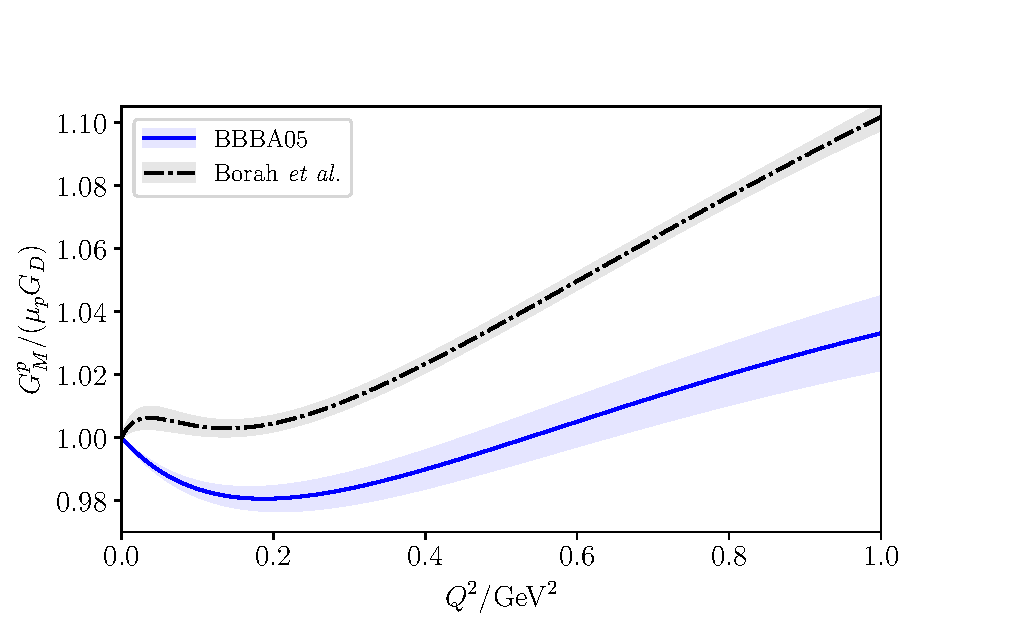
\includegraphics[width=0.7\textwidth]{plots/proton_magnetic-standalone.pdf}
 \vspace{4pt}
\caption{
Proton magnetic form factor normalized by a reference dipole ansatz
with a dipole mass of $0.84~{\rm GeV}$.
This plot is reproduced from Fig.~4 in Ref.~\cite{Borah:2020gte}
 and the associated supplemental data.
The proton-only fit to a $z$-expansion by Borah {\it et al.}~\cite{Borah:2020gte}
and the BBBA05 parameterization~\cite{Bradford:2006yz} are shown.
\label{fig:protonmagneticff}
}
\end{figure}
%------------------------------------------------------------------------------

However, there is a significant tension in existing parameterizations of the proton magnetic form factor, as
shown in Figure~\ref{fig:protonmagneticff}.
Two different parameterizations of the form factor, normalized by the dipole, are shown.%
\begin{marginnote}
\entry{BBBA05}{The Bradford, Bodek, Budd and Arrington 2005 nucleon elastic form factor parameterization~\cite{Bradford:2006yz}}
\end{marginnote}%
The BBBA05~\cite{Bradford:2006yz} are displayed as the lower (blue) band with a solid mean value.
A more recent $z$-expansion parameterization from Borah {\it et al.}~\cite{Borah:2020gte} is displayed by the upper (black) band with a dashed mean value.
The tension is significant over all $Q^2 > 0$, at the level of several percent,
including significant disagreement in the slope of the form factor at $Q^2 = 0$.
Of the nucleon form factor calculations from LQCD,
the vector form factors are also the most mature,
exhibiting no obvious tensions with experimental determinations
of the vector form factors at their current level of precision.
A percent level calculation of the form factor $Q^2$ behavior combined with a direct calculation of the slope of the magnetic form factor would provide useful insight about this tension or could discriminate
between the two parameterizations.

The nucleon axial form factor has had a much more complicated past than the vector form factors in LQCD.%
\begin{marginnote}
 \entry{Axial charge} {The axial form factor at zero momentum transfer, $g_{\mathrm{A}} = F_{\mathrm{A}}(0)$}
\end{marginnote}%
The axial charge is a key benchmark for LQCD and is precisely known
from neutron decay experiments~\cite{Dubbers:2021wqv}.
LQCD calculations of the axial charge have historically been low compared to experiment~\cite{Aoki:2021kgd},
 and the discrepancy has been the topic of some controversy.
It is now understood that the treatment of excited state systematics is the main culprit for this discrepancy~\cite{Bar:2017kxh,Ottnad:2020qbw,Aoki:2021kgd}.
With proper control over the excited state contamination, the LQCD calculations are now in good agreement with the experimental value~\cite{Jang:2019vkm,Gupta:2018qil,Alexandrou:2020okk,Abramczyk:2019fnf,Park:2021ypf,RQCD:2019jai,Hasan:2019noy,Djukanovic:2021yqg,Harris:2019bih,Liang:2018pis,Shintani:2018ozy,Ishikawa:2018rew}
 with one group achieving a sub-percent determination of $g_{\mathrm{A}}$~\cite{Chang:2018uxx,Berkowitz:2018gqe,Walker-Loud:2019cif}.

Armed with the newfound confidence in the control of systematics for the axial charge,
 more emphasis is now being put into the form factor at nonzero momentum transfer
to make contact with the needs of the neutrino community and provide
 complementary constraints on free nucleon amplitudes.
One extremely striking feature of LQCD calculations is the strong preference for a slower
fall off of the form factor with increasing $Q^2$ than predicted by phenomenological determinations from experiment (Figure~\ref{fig:gaq2_overlay}).
This preference is consistently reproduced by several lattice collaborations using
independent computation methods, lending more credence to the result.
When integrated over the full range of $Q^2$ to compute the nucleon cross section,
this translates to an enhancement in the free nucleon cross section as large as 30--40\%
over neutrino energies greater than $1~{\rm GeV}$ (Section~\ref{sec:impact}).
In addition, the precision on the axial form factor uncertainty from LQCD
is small enough to be sensitive to the tension between vector form factor parameterizations.

The aforementioned situation with nucleon form factors is depicted in Figure~\ref{fig:nucleonxsec}.
The labels correspond to the following form factor parameterization choices and uncertainties:
\begin{description}
 \item[BBBA05] Vector form factors from BBBA05~\cite{Bradford:2006yz},
 and axial form factors from Meyer~{\it et al.}~\cite{Meyer:2016oeg}.
 The uncertainty is taken from BBBA05, with all fit parameters assumed to be uncorrelated.
 \item[$z$ exp, vector] Vector form factors from Borah~{\it et al.}~\cite{Borah:2020gte},
 and axial form factors from Meyer~{\it et al.}~\cite{Meyer:2016oeg}.
 The uncertainty is taken from Borah~{\it et al.}
 \item[$z$ exp, ${\rm D}_{2}$ axial] as ``$z$ exp, vector,''
 with the uncertainty taken from Meyer~{\it et al.} instead.
 \item[$z$ exp, LQCD axial] Vector form factors from Borah~{\it et al.}~\cite{Borah:2020gte},
 axial form factors and their uncertainty provided by authors from an LQCD simulation
 on a single physical mass ensemble.
\end{description}
Of particular note is the observed tension between the black and blue bands,
 which results from the tension between proton magnetic form factor parameterizations
 (see Figure~\ref{fig:protonmagneticff}).
The size of the red band with respect to the green band demonstrates the uncertainty reduction from replacing the deuterium scattering axial form factor with one obtained from LQCD, and the significant change in normalization is due to the slower fall off of the axial form factor.
Additionally, the size of the red band demonstrates the relevance of the tension in vector form factors, characterized by the difference between the black and blue curves.

%The black dot-dashed curve is the default case, which uses the $z$ expansion parameterizations of the vector and axial form factors from Refs.~\cite{Borah:2020gte}~and~\cite{Meyer:2016oeg}, respectively.
%The green band shows the uncertainty obtained from the axial form factor alone, and the gray band from the (much smaller) vector form factor uncertainty by itself.
%The blue solid curve substitutes the vector form factors of the default choice with the BBBA05 parameterization~\cite{Bradford:2006yz}, taking the uncorrelated uncertainty from the BBBA05 vector form factors only.
%The observed tension between the black and blue bands is the result of the tension between proton magnetic form factor parameterizations (see Figure~\ref{fig:protonmagneticff}).
%The red dotted curve instead substitutes the axial form factor of the default with a parameterization obtained from lattice QCD and its uncertainty.
%The size of the red band with respect to the green band demonstrates the uncertainty reduction from replacing the deuterium scattering axial form factor with one obtained from LQCD, and the significant change in normalization is due to the slower fall off of the axial form factor.
%Additionally, the size of the red band demonstrates the relevance of the tension in vector form factors, characterized by the difference between the black and blue curves.


%------------------------------------------------------------------------------
% nu-N cross section
\begin{figure}[hbt!]
 \centering
 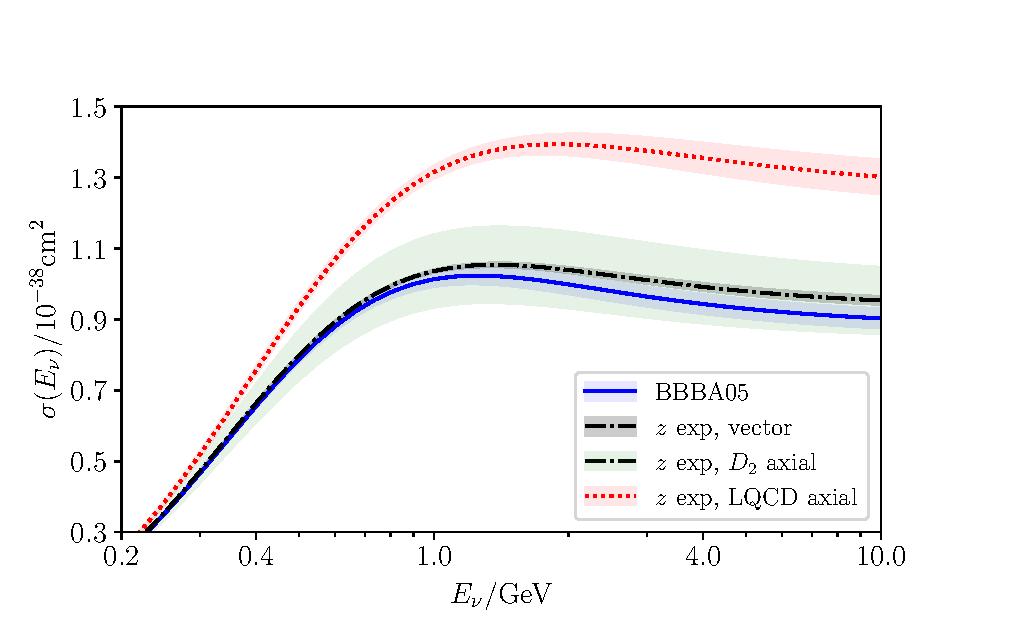
\includegraphics[width=0.7\textwidth]{plots/xsec_comparison-standalone.pdf}\vspace{4pt}
\caption{
 Neutrino cross sections on a free neutron, with their uncertainty bands,
 for various choices of parameterization.
 The curves labeled ``BBBA05'' (blue solid line, Ref.~\cite{Bradford:2006yz})
 and ``$z$ exp, vector'' (black dot-dashed line, Ref.~\cite{Borah:2020gte}) use the
 $z$ expansion axial form factor from Ref.~\cite{Meyer:2016oeg},
 with only the uncertainty from the vector form factors plotted
 to highlight the tension between the parameterizations shown in Fig.~\ref{fig:protonmagneticff}.
 The same form factor parameterizations are used for both ``$z$ exp, vector'' and
 ``$z$ exp, D$_{2}$ axial'' (green dot-dashed line)
 but in the latter case the uncertainty band is taken only from
 the axial form factor rather than only from the vector form factor.
 The red dotted line labeled ``$z$ exp, LQCD axial'' is parameterized by
 the vector form factors of Ref.~\cite{Borah:2020gte} with no uncertainty
 and the axial form factor with its uncertainty taken from LQCD.
 \label{fig:nucleonxsec}
}
\end{figure}

%\cw{I think these comments are out of place here. They should be removed or worked into the intro or the next section.}
%In the next section, we review the current status of LQCD calculations of the axial form factor.
%We emphasize that LQCD calculations of the electric and magnetic form factors are more mature, but equally important.
%We anticipate, given the state of the field, that within a couple years, we will have a complete error budget for the single nucleon (quasi-) elastic form factors from LQCD.
%
%
%\bigskip\noindent{\color{red}comments below:}
%\begin{description}
%\item[first $z$ exp vector form factor] \cite{Ye:2017gyb}
% - does not use constraints from muonic hydrogen, many more fit parameters
%\item[Vector form factor tensions] \cite{Borah:2020gte}
%\item[Muonic hydrogen review] \cite{Hill:2017wgb}
%\end{description}
%
%\textcolor{red}{[Most focus on axial, but vector is important too]}
